\documentclass[12pt]{article}

\title{AlgoBowl Software Design}
\date{24 April 2017}
\author{Jack Rosenthal}

\usepackage{fontspec}
\usepackage{hyperref}
\usepackage[margin=25mm]{geometry}
\usepackage{wasysym}
\usepackage{float}

\newcommand\ctrltitle[1]{\par\medskip\texttt{\large #1}\\}
\newcommand\ctrlauth[1]{Authorization: #1\\}
\newcommand\ctrldesc[1]{$\rhd$ \textsl{#1}\par\medskip}

\setlength\parindent{0pt}
\setlength\parskip{5pt plus 1pt minus 1pt}

\begin{document}

\maketitle

\section{Introduction}

AlgoBowl is an extension to the CS CONNECT web application used in CSCI-406:
Algorithms. Students are given a NP-hard problem to solve by the professor and
work in small groups (typically of three students) to create and implement a
heuristic to get the best solution they can. Once they have done this, each of
the groups:
\begin{enumerate}
    \item Designs an input for the other groups to run and uploads it to the
        AlgoBowl webpage
    \item Downloads all the inputs from the other groups and runs it on their
        program
    \item Uploads their outputs for the corresponding inputs
    \item Verifies each of the outputs for their input and marks it as either
        \emph{Accepted} or \emph{Rejected}
\end{enumerate}

To keep the process flowing, the students are given deadlines they need to
complete each of these steps by.

At the end of the assignment, each of the students are given an opportunity to
rank their fellow team members' efforts as a percentage. The instructor then
downloads these effort percentages and assigns grades to each student.

\section{Database Model Design}

Figure \ref{erd} shows a (Peter Chen style) entity relationship diagram showing
the different database models that should be used to implement the software.

\begin{figure}
    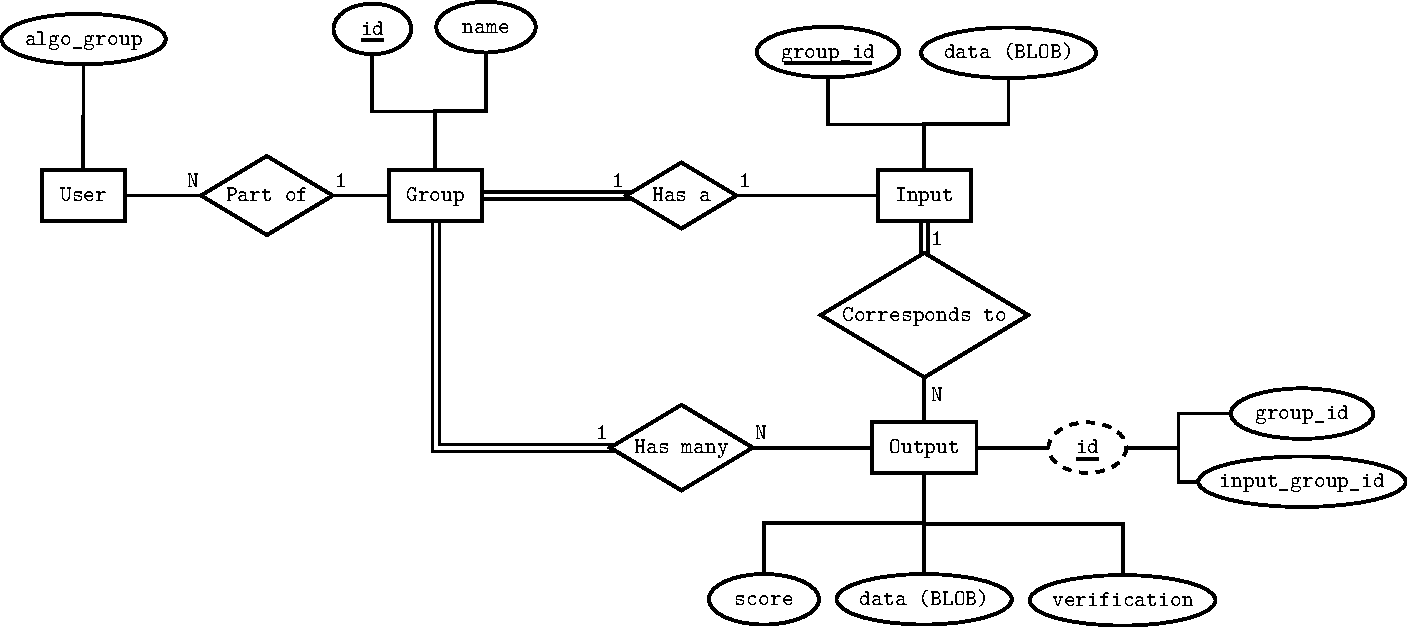
\includegraphics[width=\textwidth]{graphics/algo_erd.pdf}
    \caption{The database model}
    \label{erd}
\end{figure}

Notice the following:

\begin{itemize}
    \item The attribute \texttt{algo\_group} as an extension of the CONNECT
        \texttt{User} model specifies the group ID that the student is a
        participant of.  For students not enrolled in CSCI-406, this attribute
        is simply set to a \texttt{NULL} value.
    \item The \texttt{Group} model relates the numerical group ID to the team's
        name. Only the instructor may have means of discovering both sides of
        this relation as the names of the students in each group are not
        anonymous but their results must be.
    \item Both the \texttt{Input} and \texttt{Output} models store the binary
        data that is uploaded. \textbf{This data is not stored on the
        filesystem!}
    \item The \texttt{Output} model contains both a \texttt{score} attribute
        and a \texttt{data} attribute. When an output is uploaded, the first
        line is separated from the remainder of the file and parsed as a
        numerical value. This is explained further later on in the controller
        logic.
    \item The primary key if the \texttt{Output} model is the combination of
        both the group that uploaded the output and the group that the input
        corresponds to. There is no \texttt{id} attribute.
    \item The \texttt{verification} attribute of the \texttt{Output} model is a
        enumerable type; being one of \emph{Waiting}, \emph{Accepted}, or
        \emph{Rejected}.
\end{itemize}

There are two more models which do not have relations to the other AlgoBowl
models: the \texttt{Evaluation} model (shown in Figure \ref{evaltable}) and the
\texttt{AlgoBowlConfiguration} model (shown in Figure \ref{conftable}).

\begin{figure}
    \centering
    \textbf{Evalutions} \\
    Primary key: (\texttt{from\_user\_id}, \texttt{to\_user\_id}) \\
    Foreign key constraints: \\
    \texttt{from\_user\_id} $\to$ \texttt{User.id} \\
    \texttt{to\_user\_id} $\to$ \texttt{User.id} \\
    \begin{tabular}{| c | c | c |}
        \hline
        \texttt{from\_user\_id} & \texttt{to\_user\_id} & \texttt{effort} \\
        \hline
        1 & 1 & 35 \\
        \hline
        1 & 2 & 35 \\
        \hline
        1 & 3 & 30 \\
        \hline
        $\vdots$ & $\vdots$ & $\vdots$ \\
        \hline
    \end{tabular}
    \caption{The Evalutions Table}
    \label{evaltable}
\end{figure}

The configuration table is a Berkeley DB style table containing the
configuration options for the current AlgoBowl problem. This table stores
weather this problem is a minimization or maximization problem, as well as any
other associated data for the problem.

\begin{figure}
    \centering
    \textbf{AlgoBowlConfiguration} \\
    \begin{tabular}{| c | c |}
        \hline
        \texttt{key} & \texttt{value} \\
        \hline
        \texttt{problem\_type} & \texttt{min} \\
        \hline
        \texttt{instructor} & \texttt{dmehta@mines.edu} \\
        \hline
        $\vdots$ & $\vdots$ \\
        \hline
    \end{tabular}
    \caption{The Configuration Table}
    \label{conftable}
\end{figure}

\clearpage

\section{Controller Design}

\ctrltitle{GET algobowl}
\ctrlauth{CS CONNECT User}
\ctrldesc{Generate the rankings page}

When the landing page for AlgoBowl is loaded, a table of rankings is shown to
the user. This rankings table is accessible \emph{regardless of weather the
current user is a CSCI-406 student} to allow others to look in at the progress
of AlgoBowl.

An example table is shown in Figure \ref{algotbl}. In this table:
\begin{itemize}
    \item A ranking of \textsf{N} indicates that the output was not submitted yet
    \item A ranking of \textsf{R} indicates that the output was rejected
    \item A ranking of a number with a \textsf{(W)} next to it indicates the output is waiting for acceptance
    \item A ranking of a number without a \textsf{(W)} next to it indicates the output was accepted
    \item Groups highlighted in red have at least one rejected output
    \item Groups highlighted in orange have at least one output they have not submitted yet
    \item Groups highlighted in green have all their outputs accepted
\end{itemize}

\begin{figure}
    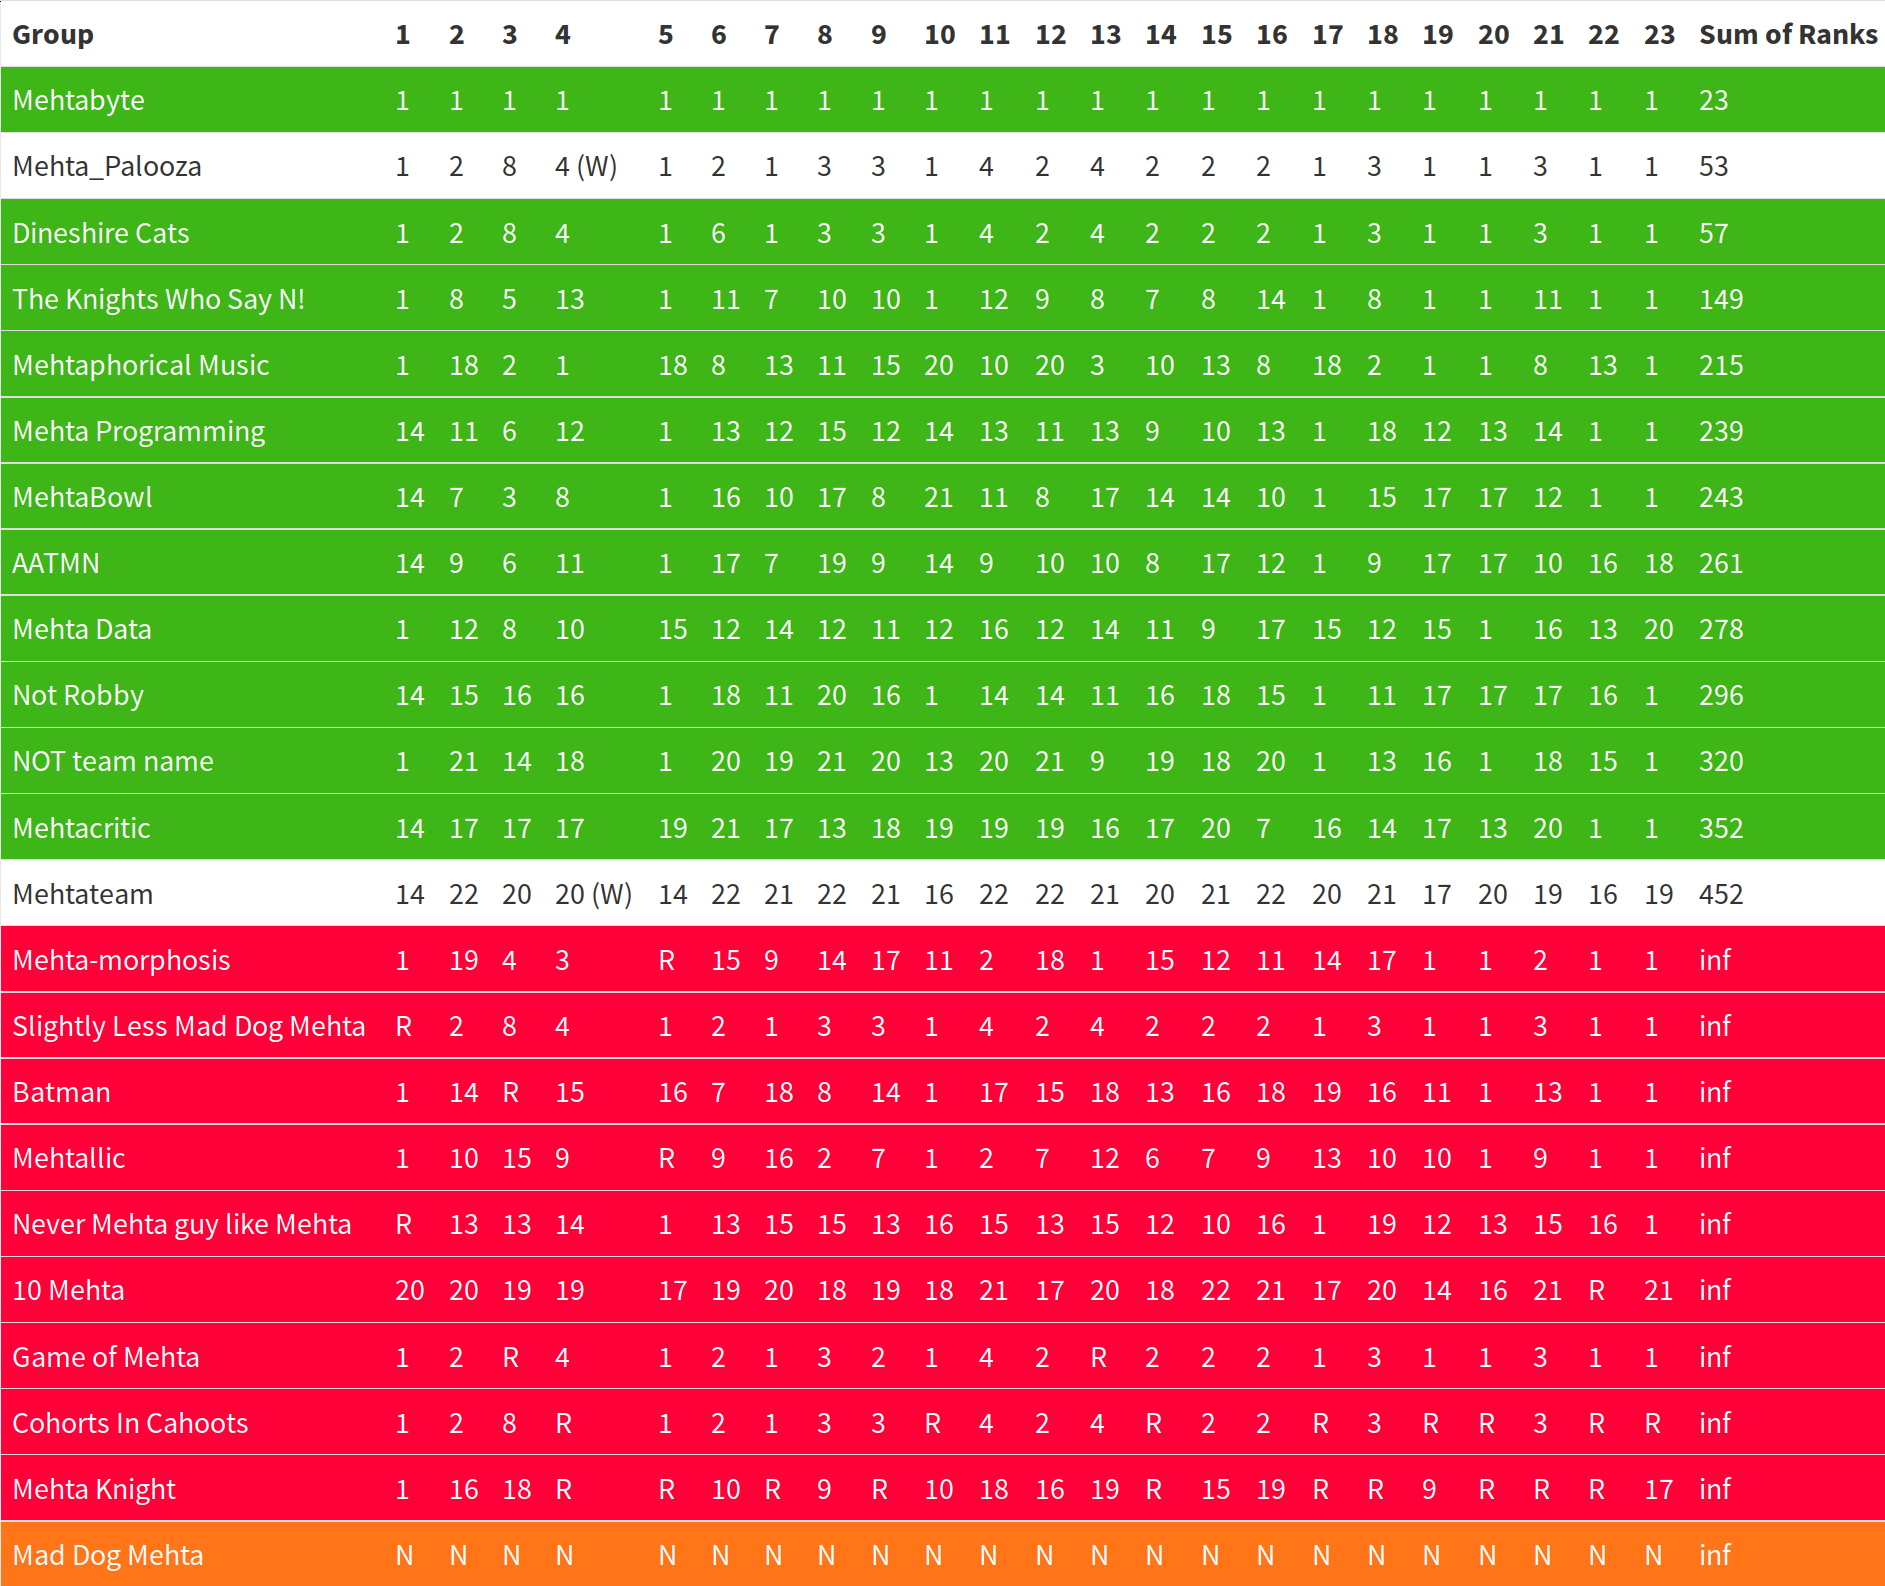
\includegraphics[width=\textwidth]{graphics/algotbl}
    \caption{An AlgoBowl Rankings Table}
    \label{algotbl}
\end{figure}

A few important notes on how this table was generated:

\begin{itemize}
    \item For a particular input, if any teams tie, they should share the same
        rank and the ranks of all the teams should offset accounting for the
        number of tied ranks. For example, if two teams tie for first place,
        the next place is third place, not second. In other words, if $N$ teams
        did better on a particular input, then the rank of that team for the
        input is defined to be $N + 1$.
    \item When a team has rejected outputs or has not uploaded all of their
        outputs, they cannot receive a finite value for sum of ranks, because
        they have not yet completed the competition.
    \item When a team has not had their output accepted yet, they can be given
        a rank compared to the others, but the table should indicate it is not
        accepted yet.
    \item When two teams tie for their sum of ranks, a reasonable secondary
        sorting key should be used to show their order in the table. This
        secondary key (sorted by minimum) is calculated as $R - 2A - W$, where $R$
        is the number of rejected outputs for that team, $A$ is the number of
        accepted outputs for that team, and $W$ is the number of outputs
        waiting acceptance for that team. In the case that this secondary sort
        key is equivalent as well, the group's number is used as the third key.
    \item Group numbers should not be shown next to their scores (but instead
        their group name), as this preserves student anonymity.
\end{itemize}

\ctrltitle{GET algobowl/submission}
\ctrlauth{AlgoBowl Student}
\ctrldesc{Generate the Team Name Change, Input/Output Upload, and Input Download Page}

\ctrltitle{POST algobowl/set\_team\_name}
\ctrlauth{AlgoBowl Student}
\ctrldesc{Handle form submission to change team name}

Makes sure the team name is valid and less than 20 characters, and sets the
team's name. Redirects back to the inputs page.

\ctrltitle{POST algobowl/upload\_input}
\ctrlauth{AlgoBowl Student}
\ctrldesc{Handle form submission to upload the group's input}

\begin{enumerate}
    \item Converts input to UNIX file format (if in MS-DOS or Mac OS format)
    \item If they are replacing a previous input:
        \begin{enumerate}
            \item Email all groups who have already submitted outputs and let
                them know they will need to redo their input and upload again.
                The text for this email is shown in Figure
                \ref{emailredo}.\footnote{This is not a catch-all solution for
                preventing outputs that don't correspond to the correct input
                (a student could still download an input, the other group
                changes their input, then the student uploads their output),
                but it's the best we can do without having students put unique
                ID's at the top of their inputs and outputs.}
            \item Delete any outputs which have already been submitted
        \end{enumerate}
    \item Store their input in the database
\end{enumerate}

\begin{figure}[H]
\begin{verbatim}
To: student1@mines.edu, student2@mines.edu, student3@mines.edu
From: algobowl@connect.mines.edu
Reply-To: instructor@mines.edu
Subject: [AlgoBowl] New Input Uploaded for Group {{Group ID}}

Dear {{Team Name}},

Group {{Group ID}} has just uploaded a new input on AlgoBowl and your
team had an output submitted already.

Your old output has been deleted. At your convenience, please download
their new input, rerun your program on it, and upload the new output.

Best regards,

The AlgoBowl System
\end{verbatim}
    \caption{The email to be sent when an output redo is needed}
    \label{emailredo}
\end{figure}

\ctrltitle{GET algobowl/input/input\_group\_\{group\_id\}.txt}
\ctrlauth{AlgoBowl Student or AlgoBowl Admin}
\ctrldesc{Download input for group \texttt{group\_id}}

If Group \texttt{group\_id} has not uploaded an input yet, this page should
abort with a 404 error.

\ctrltitle{GET algobowl/all\_inputs.zip}
\ctrlauth{AlgoBowl Student or AlgoBowl Admin}
\ctrldesc{Generate a ZIP archive of all the inputs for the user}

\ctrltitle{POST algobowl/upload\_output}
\ctrlauth{AlgoBowl Student}
\ctrldesc{Handle form submission to upload the group's output}

Takes a parameter of the input Group ID the output corresponds to. This should:

\begin{enumerate}
    \item Converts the output to UNIX file format (if in MS-DOS or Mac OS format)
    \item Strip the first line off the output and convert it to a numerical
        type. This is the \texttt{score} attribute. If this process fails, it
        should raise an error to the user.
    \item Store the remainder of the output as the \texttt{data} attribute
    \item Set the \texttt{verification} attribute to \emph{Waiting}
    \item Store their output in the database
\end{enumerate}

\ctrltitle{GET algobowl/verification}
\ctrlauth{AlgoBowl Student}
\ctrldesc{Generate a page with output download links and a button to accept or
reject each of them}

\ctrltitle{GET algobowl/output/output\_from\_\{from\_id\}\_to\_\{to\_id\}.txt}
\ctrlauth{AlgoBowl Student with Group ID \texttt{to\_id} or AlgoBowl Admin}
\ctrldesc{Download output from group \texttt{from\_id} to group
\texttt{to\_id}}

\ctrltitle{GET algobowl/all\_outputs\_to\_\{to\_id\}.zip}
\ctrlauth{AlgoBowl Student with Group ID \texttt{to\_id} or AlgoBowl Admin}
\ctrldesc{Generate a ZIP archive of all the outputs to group \texttt{to\_id}}

\ctrltitle{GET algobowl/evaluations}
\ctrlauth{AlgoBowl Student}
\ctrldesc{Generate student evaluations page}

\ctrltitle{POST algobowl/evaluations}
\ctrlauth{AlgoBowl Student}
\ctrldesc{Set AlgoBowl Evaluations for a certain student}

This controller method should verify the submitted evaluations sum to exactly
100, and raise an error otherwise.

\ctrltitle{GET algobowl/setup}
\ctrlauth{AlgoBowl Admin}
\ctrldesc{Geterate AlgoBowl Setup Page}

\ctrltitle{POST algobowl/setup}
\ctrlauth{AlgoBowl Admin}
\ctrldesc{Process a new AlgoBowl setup}

This method should:
\begin{enumerate}
    \item Reset AlgoBowl, clearing any previous data
    \item Set up the new AlgoBowl with the specified teams and configuration
\end{enumerate}

\ctrltitle{GET algobowl/verif\_editor}
\ctrlauth{AlgoBowl Admin}
\ctrldesc{Generate verification editing page for the admin}

\ctrltitle{POST algobowl/verif\_editor}
\ctrlauth{AlgoBowl Admin}
\ctrldesc{Process a verification edit for the admin}

\ctrltitle{GET algobowl/eval\_admin}
\ctrlauth{AlgoBowl Admin}
\ctrldesc{View evaluations}

\ctrltitle{GET algobowl/evaluations.csv}
\ctrlauth{AlgoBowl Admin}
\ctrldesc{Download a CSV file with the evaluations}

\section{Interface \& View Design}

\subsection{Tabs}

For students, the tabs should read:

\texttt{Rankings | Submission | Verification | Evaluations}

For admins, the tabs should read:

\texttt{Rankings | Submission | Verification Editor | View Evaluations | Setup}

For users who are not logged in, they should be able to view the rankings page,
but instead of the tabs there is a message:

\emph{You are not currently enrolled on an AlgoBowl team. If you think you have
received this message in error, please contact your instructor.}

\subsection{Rankings}

The rankings page should view like Jack's prototype: \\
\url{https://mastergo.mines.edu/cgi-bin/algotbl.cgi}

Note that the view for this page from the old AlgoBowl will likely not be
anyhow salvageable, as it is far different from Jack's prototype.

\subsection{Submission}

The submission page should be like the one on the current AlgoBowl: \\
\url{https://mastergo.mines.edu/csconnect-oldprod/algobowl/submission}

It should also include a link to download all inputs as a ZIP file.

For the admin user, do not show the Input Upload or Change Team Name sections.

\subsection{Verification}

The verification screen should look like the one on the current AlgoBowl: \\
\url{https://mastergo.mines.edu/csconnect-oldprod/algobowl/verification}

It should also include a link to download all outputs for that team as a ZIP
file.

\subsection{Evaluation}

The evaluation screen should look like the one on the current AlgoBowl: \\
\url{https://mastergo.mines.edu/csconnect-oldprod/algobowl/evaluations}

\subsection{Verification Editor}

The verification editor screen should present the admin with a matrix of
verifications (text boxes containing A, R, or W) and allow the admin to edit
the verifications and resubmit the page.

\subsection{View Evaluations}

The evaluations page should show a table of all evaluations to the admin as
well as a button to download a CSV file.

\subsection{Setup}

A warning should appear on this page:

\emph{Submitting this form will setup AlgoBowl for a new semester, deleting all
current AlgoBowl data}

The admin should be able to design teams and select between a minimization or
maximization problem.

\end{document}
